\documentclass[document.tex]{subfiles}
\begin{document}

\chapter{Metody równoległego przetwarzania danych}

\section{Wielowątkowość aplikacji dla języka C/C++}
%wstęp równoległość
\indent Najbardziej popularnym podejściem do pisania aplikacji jest sekwencyjne wykonywanie
instrukcji przez procesor - tylko jedna z nich może być wykonywana w tym samym czasie.
Jednak dużą ilość problemów można rozbić na niezależne fragmenty,
które mogą być rozwiązywane równolegle. Obecnie powszechnie stosowane procesory wielordzeniowe dają możliwość rozdzielenia obciążenia obliczeniowego na poszczególne rdzenie oraz dla każdego rdzenia na osobne wątki.\cite{Computer_Architecture_Patterson_Hennesy}\cite{Parallel_computing_article} \\
 %wątek def i opis
 \indent Wątek jest to podproces, który posiada własny stos, zestaw rejestrów, ID, priorytet i wykonuje określony fragment kodu programu. 
 W przeciwieństwie do prawdziwego procesu posiada wspólną pamięć globalną i sterty, dzieloną z innymi wątkami istniejącymi w ramach tego samego procesu. 
 Wątki procesu wykonują się równolegle, dopóki nie potrzebują dostępu do zasobów we wspólnej pamięci.\cite{POSIX_article}\cite{POSIX_tutorial} 
 Wtedy ze względu na problem błędnego odczytu, bądź zapisu wartości w pamięci kiedy inny wątek ją już nadpisał, może spowodować niewłaściwe działanie programu. 
 Fragmenty kodu gdzie może dojść do tego problemu nazywane są sekcjami krytycznymi. Do zabezpieczania sekcji krytycznych programu stosowane są blokady - muteksy(Mutual exclusions) oraz zmienne warunkowe.
 Zastosowanie muteksa powoduje, że w danym momencie tylko jeden wątek może wykonywać kod chroniony przez tą blokadę i dopóki nie opuści chronionej sekcji krytycznej inny wątek nie może zacząć jej wykonywać. 
 Zmienne warunkowe stosowane są do sygnalizowania postępu danego wątku, tak aby inny mógł kontynuować wykonywanie operacji sekcji krytycznej. 
 Stosowane razem z blokadami umożliwiają właściwą synchronizację pracy wątków tego samego procesu.
\cite{POSIX_Butenhof}\cite{C++_Stroustrup} \\
 %watek - wady i zalety 
\indent Używanie wielowątkowości w aplikacjach pozwala na wykorzystanie możliwości sprzętowych procesorów wielordzeniowych do obliczeń równoległych.
Ponadto wielowątkowy model programowania umożliwia wykonywanie przez proces dalszych działań w czasie czasochłonnych obliczeń, bądź czekania na zdarzenie blokujące - takie jak ,np.sygnał z urządzenia peryferyjnego.
Wadą tworzenia dodatkowych wątków w programie jest narzut obliczeniowy
związany z ich synchronizacją(omawiany wcześniej problem wyścigu oraz zjawisko zakleszczenia - wątki czekają na siebie nawzajem żeby móc kontynuować obliczenia) oraz dostępem do wspólnego obszaru pamięci.\cite{POSIX_Butenhof}\cite{C++_Stroustrup} \\
%podsumowanie
\indent W tym rozdziale zostaną omówione różne metody tworzenia aplikacji
wielowątkowych w języku C/C++. Skupiono się na bibliotekach dla tych języków
programowania ze względu na ich popularność w tworzeniu rozwiązań dla systemów wbudowanych, która wynika z wysokiej wydajności kodu i małego zużycia pamięci w porównaniu do języków interpretowanych, np. Java, Python.\cite{C++_Stroustrup}\cite{C_King}

\subsection{Biblioteka POSIX dla systemów Unix}
\indent Dla systemów z rodziny Unix w 1995 ustalony został standard programowania 
wielowątkowego nazywany POSIX threads, w skrócie Pthreads. API Pthreads zostało zdefiniowane jako zestaw typów i procedur w języku C, zawarte w pliku nagłówkowym
\code{<pthread.h>} i bibliotece libpthread.\cite{POSIX_article}
Korzystanie z biblioteki Pthreads do tworzenia wątków generuje mniejszy narzut
niż tworzenie osobnych procesów do równoległego przetwarzania danych.\cite{POSIX_article} 
\\
\indent Wątek w programie jest reprezentowany poprzez zmienną typu \code{pthread\_t}, 
najczęsciej zdefiniowaną jako zmienna statyczna lub jako struktura, która jest zaalokowana na stercie.\cite{POSIX_Butenhof}\cite{POSIX_article}\cite{POSIX_tutorial} 
Do każdego stworzonego wątku przypisana jest funkcja, którą będzie wykonywał.
Funkcja powinna przyjmować jako argument zmienną wskaźnikową \code{void*} i zwracać
wartość tego samego typu. Za tworzenie nowego wątku odpowiedzialna jest funkcja \code{pthread\_create}. Przyjmuje ona adres funkcji oraz argument z jakim ma zostać wywołana.
Wywołanie \code{pthread\_create} oprócz rozpoczęcia nowego wątku zwraca identyfikator
\code{pthread\_t}, który będzie wykorzystywany do odnoszenia się do stworzonego wątku.
Wątek zostaje zakończony jeśli wykona wszystkie instrukcje swojej funkcji lub jeśli wywoła procedurę \code{pthread\_exit}. \cite{POSIX_Butenhof}

\begin{figure}[h]
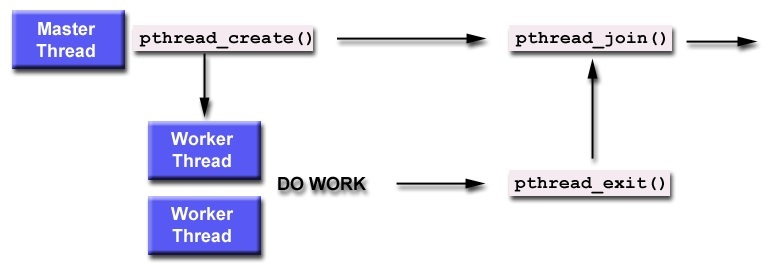
\includegraphics[scale=0.7]{posix_thread_tree}
\caption{Wykorzystanie \code{pthread\_join} do synchronizacji wątków\protect\cite{POSIX_article}}
\label{fig:inspekcja}
\end{figure}

Jedną z podstawowych metod synchronizacji pomiędzy wątkami jest użycie funkcji \code{pthread\_join}, która powoduje zatrzymanie dalszego wykonywania instrukcji dopóki stworzony wątek nie zakończy pracy.
Tylko wątki, które został stworzone z atrybutem \code{joinable}, 
a nie \code{detached}(odłączony) mogą używać tego rodzaju synchronizacji.\cite{POSIX_article}(patrz \ref{lst:basic_thread}). % kontynuować o wątkach
\\
\lstinputlisting[language=C, label={lst:basic_thread}, caption=Przykład tworzenia i uruchamiania wątków]{code_snippets/posix_example_0.c} 

\indent W celu zapewnienia bezpieczeństwa w współdzieleniu zasobów
pomiędzy wątkami podczas wykonywania sekcji krytycznych,
najpopularniejsze jest wykluczenie jednoczesnego czytanie bądź zapisu
wartości w dzielonej pamięci. Używane do tego są zmienne wzajemnego
wykluczenia - w skrócie muteks(mutual exclusion). Muteks jest szczególnym przypadkiem semaforu Dijkstry - semaforem binarnym 
o zbiorze wartości {0, 1}.\cite{POSIX_Butenhof}\cite{POSIX_tutorial}\cite{POSIX_article} 
W bibliotece POSIX threads muteks jest reprezentowany jako zmienna typu \code{pthread\_mutex\_t}. W celu posiadania globalnego
zasięgu deklarowana jest jako zmienna \code{static} lub \code{extern}.
\cite{POSIX_Butenhof}\cite{C_King}(patrz\ref{lst:mutex_thread})
W celu deklaracji muteksa wykorzystywane jest makro \code{PTHREAD\_MUTEX\_INITIALIZER}(patrz . Jeśli muteks jest używany jako
element dynamicznie alokowanej struktury, musi zostać zainicjalizowany 
wywołaniem funkcji \code{pthread\_mutex\_init}. Ponadto musi być w ten
sposób inicjalizowany, jeśli nie ma posiadać domyślnych atrybutów.
Niezbędne jest po zakończeniu używania muteksa, zwolnienie zaalokowanej pamięci, poprzez wykorzystanie funkcji \code{pthread\_mutex\_destroy}.\cite{POSIX_Butenhof} 
\\
\lstinputlisting[language=C, label={lst:mutex_thread}, caption=Przykład wykorzystanie muteksa do synchronizacji
aplikacji wielowątkowej]{code_snippets/posix_example_1.c}

\indent Pthreads do komunikacji pomiędzy wątkami wykorzystuje zmienne
warunkowe(condition variables), które mają informować o stanie 
współdzielonych zasobów. Używane razem z muteksami, w atomiczny 
sposób zwalniają blokadę sekcji krytycznej, dopóki inny wątek nie
zasygnalizuje kontynuacji używając funkcji \code{pthread\_cond\_signal}. Dzięki temu inny wątek może kontynuować pracę 
zanim zostanie wykonana chroniona sekcja krytyczna.

\indent Dzięki przedstawionym metodom sygnalizacji stanu oraz 
blokadom, możliwe jest zaprojektowanie pożądanego podziału obciążenia
obliczeniowego. Biblioteka POSIX, choć wiekowa dalej jest stosowana
dzięki małemu narzutowi(napisana w języku C), obszernej dokumentacji 
oraz dużej ilości starego kodu, który dalej jest stosowany w nowych
rozwiązaniach systemów wbudowanych i czasu rzeczywistego.\cite{POSIX_tutorial}
\clearpage
%%%%%%%%%%%%%%%%%%%%%%%%%%%%%%%%%%%%%%%%%%%%%%%%%%%%%%%%%%%%%%%%%%%
\subsection{OpenMP - wieloplatformowe API}
To jest podrozdział 2 rozdziału 1
\cite{openmp_pacheco}
\cite{openmp_spec}
\cite{openmp_guide}
\cite{openmp_slides}

\subsection{Wielowątkowość w standardzie C++11}
To jest podrozdział 3 rozdziału 1


%%%%%%%%%%%%%%%%%%%%%%%%%%%%%%%%%%%%%%%%%%%%%%%%%%%%%%koniec rozdziału


\section{Programowanie równoległe z wykorzystaniem GPU}
To jest rozdział 2

\subsection{Architektura GPU i porównanie względem CPU}
To jest podrozdział 1 rozdziału 2

\subsection{Biblioteka OpenCL}
To jest podrozdział 2 rozdziału 2

%ewentualnie można coś dodać o CUDA jeśli objętościowo będzie za cienkie
\end{document}
